\chapter{Case}
%%%%%%%%%%
\section{Organizational Setting}
This thesis comes into being as part of the \textit{ERCIS Omni-channel lab powered by Arvato}. This cooperation fosters research in omni-channel CRM through cooperation with Arvato, a leading European outsourcing provider. The focus is set on the CRM services division, which is one of four \textit{solution groups}. While the focus is on the German market, Arvato operates international. The organizational structure can be described as decentralized in the past, but it is intended to integrate the independent country organizations more deeply within the solution group. As clients intensify international outsourcing of customer services to Arvato, a need to deliver an orchestrated outsourcing concept across borders arises. The solution group CRM therefore needs more alignment in their three constituents

\begin{itemize}
	\item Sales \& Business Development,
	\item Portfolio Management \& IT and
	\item Operations.
\end{itemize}

A discussion of organizational structures is not in scope of this work, but this view on the business helps to derive a process structure that is later used in the reference model. As an analogy to the domain of retail, one can see its supply and distribution side in form of Sales \& Business Development and Operations, respectively. The \textit{Sales \& Business Development }organization is oriented towards the outsourcing company, e.g., client. It is the main channel of communication to manage existing and potential clients and hence enables the \textit{supply} of outsourcing contracts and therefore business to the organization.\\
 \textit{Portfolio Management \& IT} organizes available service products and their technological foundation. Especially CRM platforms, their selection and implementation is part of their capabilities. With a decentralized orientation in the past, Arvato faces the problem of a heterogeneous system landscape in client business, as there was no guidance for platform selection. The aspired product orientation at Arvato demands standardization in platforms, so that a managed portfolio becomes necessary. As it is a characteristic of CRM outsourcing that clients dictate parts of the environment, \eg, technology or processes, a BPO provider needs to be flexible to react to these requirements. Interface to Sales \& Business Development are the product portfolio, which is marketed to the client. In addition, it supports in design and instantiation of products for a specific client. An internal view of products constituents, namely people, process, platform, is directed towards implementation of services and their use operational use. 
  \textit{Operations}, on the distribution side in the retail analogy, is oriented towards the customer. With call center business as core of BPO in CRM, it becomes clear that human resources are one key ingredient of the service delivery.  \\
  
  Drawing from the three described constituents of the Arvato CRM solution group, one can identify three stakeholders in the BPO provider organization. Recalling the BPO Outsourcing chain (\Fig \ref{fig:bpochain}), one part of the provider is linked to the client, another to the customer and the third is located in the center. Applying this logic to the three aforementioned units of Arvato CRM and taking a perspective that is scoped on the essential task of the unit, Sales \& Business Development targets clients and Operations is oriented towards the customer. Distancing from Arvato terminology, one can name these two stakeholders simply \textit{Sales} and \textit{Operations}. \\
  
  Portfolio Management \& IT influences both sides, as well as it acts between the two interfaces. Besides, the central part of the chain can be used to model the stakes of the BPO provider as a whole. With the taken perspective that factors out coordinating activities in the three units, the overall interest in terms of alignment across client businesses and country organizations can be captured in an isolated way. The definition of this stakeholder is necessary, as client or operations act with focus on their objectives within the organizations and put less emphasis on the provider organization as a whole. This third stakeholder is named \textit{Management}. 
  

\section{Use of a Reference Model for BPO providers in CRM}

The business model of (CRM) outsourcing providers impacts the use of a reference model in the domain. Since the outsourcing service is provided for several clients, the provider’s internal organization has to cope with this kind of diversity. Each client has its own contract and different parts of customer service process outsourced. While in general the business objects to work on (e.g., schedule in workforce management) or process steps (e.g., route incoming call) apply to all clients, they will differ on detail level (e.g., Client A will have a different routing logic as Client B and Client C has routing still in-house and outsources only after this process step).

The process differences between distinct client types of CRM outsourcing providers motivate to provide adaptive aspects in the \acrshort{RM} as described in \cite{delfmann2006adaptive}. In a configurable model the outsourcing provider can configure multiple client models based on the provided services that stay compatible and are linked with the provider model. By doing so, the provider model itself gets a reference model characteristics in the organization. \Fig \ref{fig:modelleels} visualizes the model levels. The highlighted domain reference model is center of this work. The case at Arvato represents the provider model, while businesses of Arvato can be seen as client models. By abstracting from single client business characteristics, the view of a provider is encapsulated in the empirical data that is basis of this work. It is aim and intention of the author to abstract from this provider level by means of induction and deduction from theory to derive the reference model.    

The distinction in application and reference model becomes complicated on the provider level. The model is an application of the domain reference model, hence universal validity in the domain vanishes. However, in the domain of the provider this is still valid and has a recommending character as well. With an sufficiently-large client base, diversity of client businesses is captured and therefore the universal applicability is existing to a certain extent. It is noted that sufficiently-large is no further specified here, but Arvato is seen as such a provider\footnote{Arvato is ranked the 6th largest BPO provider 2015 in terms of BPO revenue \cite{hfs2016top}. Numbers for the CRM section of Arvato are not published.}. For this work, the provider model is seen as an application model. However, usability of the reference model is of high importance. Consequently, referencing aspects on provider level are considered at construction of the domain level reference model.  
  
\begin{figure}[caption={Model levels}, label={fig:modellevels}]
	{	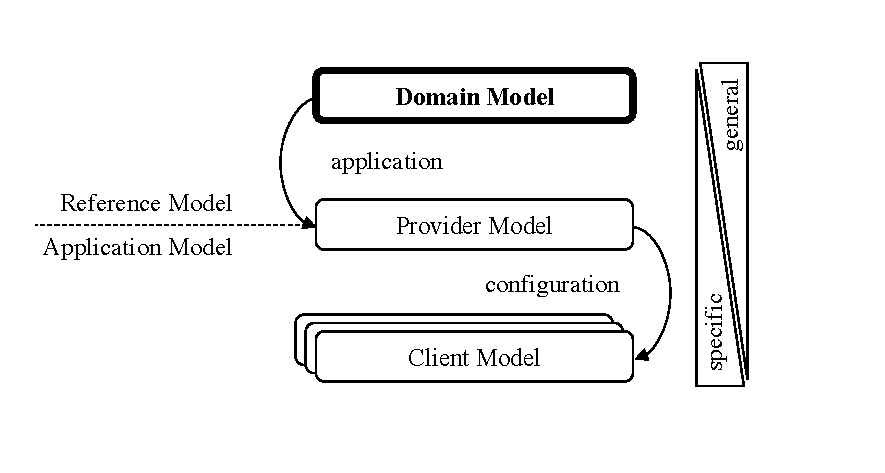
\includegraphics[width=.8\textwidth]{figures/refmodlevels.pdf}}
\end{figure}

Applying the aforementioned benefits of reference modeling \ref{sec:03_refmod} to the domain in combination with the three stakeholders, one can map these together as in \Tab \ref{tab:refmodbpobenefits}. Therefore it is mandatory to reason the benefit of reference modeling for the different stakeholders in the organization, as design science aims to solve the problem of these parties. The interplay of provider and client model impacts benefits of reference modeling in several aspects and can be attributed mainly to the benefits for Management and Operations.


% Please add the following required packages to your document preamble:
% \usepackage{multirow}
\begin{table}[caption={Benefits of Reference Modelling for BPO-providers in CRM }, label=tab:refmodbpobenefits]
	\centering
	\begin{tabular}{p{1cm} p{2cm} |p{3cm} | p{3cm} | p{3cm} |} 
		\cline{3-5}
		&                                     & \multicolumn{3}{c|}{\textbf{Stakeholder}}                                                                                                                                           \\ \cline{3-5} 
		&                                     & \textbf{Sales}                                          & \textbf{Management}                                 & \textbf{Operations}                                                 \\ \hline
		\multicolumn{1}{|l|}{\multirow{2}{*}{\textbf{Designer}}} & Knowledge                           & \multicolumn{3}{p{3cm}|}{\multirow{2}{*}{\parbox[c]{9cm}{Applicable only to researchers, not to stakeholders in the organization}}}                                                                       \\ \cline{2-2}
		\multicolumn{1}{|l|}{}                                   & Economic benefits from applications & \multicolumn{3}{l|}{}                                                                                                                                                               \\ \hline
		\multicolumn{1}{|l|}{\multirow{5}{*}{\textbf{User}}}     & Cost reduction                      & Faster client approach                                  & Reduced coordination effort                         & More efficient processes                                            \\ \cline{2-5} 
		\multicolumn{1}{|l|}{}                                   & Profit aspects                      & Organized preparation of client meetings                & Standardization facilitates better management       & Usage of new concepts leads to improvement of operational processes \\ \cline{2-5} 
		\multicolumn{1}{|l|}{}                                   & Risk reduction                      & \multicolumn{3}{l|}{\parbox[t]{9cm}{Lower risk of incorrect modeling through reference processes}}                                                                                                  \\ \cline{2-5} 
		\multicolumn{1}{|l|}{}                                   & Analysis                            & Customized offering for approached clients              & Organization-wide benchmarking                     & Benchmarking                                                        \\ \cline{2-5} 
		\multicolumn{1}{|l|}{}                                   & Information Exchange                & Structured communication of value proposition to client & Communication of best practices within organizatino & Exchange between client operations                                  \\ \hline
	\end{tabular}
\end{table}

BPO is partly cost-driven from a client perspective. For the BPO-provider low costs are therefore a necessity. Cost reduction refers to less effort in coordinating the organization through the used framework and economies of scope across client businesses. For management processes in CRM this means, that a reference process in workforce management enables a more efficient general process on provider level, while on client model level the savings are created. Client-facing processes like sales reduce costs by having a best practice process in the provider model (e.g., run consultative engagements). Operational processes like inbound call handling are always carried out for a specific client and are backbones of the BPO business. While allowing customization in client models, the compatibility to the provider model ensures the connection to reference processes.

Profit aspects often incorporate cost reduction aspects, but stand out through a significant improvement. Realization of up- and cross-selling potentials is one factor, as the necessary steps can be tightly knit into processes. Moreover, historically grown process structures both on client model level and on provider level can be identified. In the CRM domain, improved channel integration through adjusted reference processes benefits both the provider’s abilities towards omnichannel CRM and customer’s perception toward the clients’ customer service, when applied on client model level. As digital channels are becoming the dominant interaction channel, profits through analytics are more in reach.

The analysis aspect expresses the ability to compare and benchmark the business in a new way. Consistent KPI definition enables management to compare across client models, while operations is enabled to improve the analysis of employee performance, as the reference processes cover calculation rules and procedures. As cost efficiency is a primary characteristic in the BPO-field, reference modeling supports the provider’s performance management and enables more sophisticated methods through process standardization, especially with respect to more integrated customer service across channels being on the rise.

The last aspect called information exchange phrases the ability to speak a common language in the organization. In the domain of BPO-providers this is especially important, because clients vary in their terminology and beliefs of the service. A glossary is seen as an integral part of the reference model to effectively communicate meaning of business vocabulary. As different clients will show different terminology, a consistent management of a general accepted language in the provider’s organization is necessary to ensure comparability. Also, terminology can vary per geographical scope, which adds further complexity and is particularly important for global or multi-national providers. A reference model can propose guidance on this level, while custom definitions in client models will be necessary. Towards client acquisition, the models themselves can be used as basis for discussion, as well as a vehicle to communicate offered services and understanding of CRM.
%

\begin{itemize}
	\item Arvato talk in general ok
	\item servitization
	\item numbers todo
	\item history ok
	\item DSR applied here todo
	\item Refmodel use case in bpo crm todo
	\item vom Brocke grafik begründet mein Vorgehen + DSR
\end{itemize}
%%%%%%%%%%
\section{DSR Application for Arvato}

%%%%%%%%%%
\begin{itemize}
	\item wie wende ich DSR hier an?
	\item warum wende ich DSR hier an?
	\item was decke ich mich dieser arbeit ab?
	
	
\end{itemize}
%%%%%%%%%%
\section{Problem Identification}
%Activity 1. Problem identification and motivation. Define the specific research problem and justify the value of a solution. Since the problem definition will be used to develop an artifact that can effectively provide a solution, it may be useful to atomize the problem conceptually so that the solution can capture its complexity. Justifying the value of a solution accomplishes two things: it motivates the researcher and the audience of the research to pursue the solution and to accept the results and it helps to understand the reasoning associated with the researcher’s understanding of the problem. Resources required for this activity include knowledge of the state of the problem and the importance of its solution.

beschreibe das problem, was mein artefakt löst. 
relevance --> BPO Markt: 
BPO CRM RefMod
prozessmanagement ist wichtig im bpo. schewe sieht BPO sogar als synthese von outsourcing und prozessoptimierung. eben wegen dieser wichtigkeit der prozesse, sollte academics ein klareres bild von den gegebenheiten im outsourcing zeichenn. ein solches modell fehlt in der literatur. in diesem konkreten fall wird sich der domäne des bpo im crm gewidmet. es hat die besonderheit des endkundenkontakts und wird vom wandel zu einer digitalen gesellschaft stark beeinflusst. die komplexität steigt mit zunehmender vernetzung der customers. kannibalisierung im customer service bpo. 
Arvato
im anwendungsfall spielt zudem ein wandel in der organisation eine besondere Rolle. Dezentrale Stukturen, historisch gewachsen, trotzdem integrieren. herausforderungen am markt: mehr kunden verlangen internationalisierung - wie lösen mit dezentraler struktur? richtiges maß an standardisierung notwendig, einheitliche sicht aktuell schwer möglich. einheitliche terminologie

wert meiner lösung:
strukturierung der bpo prozesse.aus unternehmenssicht. grundstein in bpo in crm, aber grundstein für bpo referenzmodell  
einführung der levels zur strukturierung der provider / client sichten. erster schritt zu einem bpo referenzmodell. 
berücksichtigung von omnichannel crm. 

customer journey...

außerdem weniger faktoren, die eine dezentrale struktur rechtfertigen (bei call centern gibt es die eher). außerdem gibt es da noch mehr hebeleffekte, da weniger manuelle arbeit und es daher einfacher übergreifend einsetzbar ist. dazu muss aber alignment herrschen. produkte 
%%%%%%%%%%
\begin{itemize}
	\item Kraume interview, process interviews
	\item historisch gewachsen
	\item verschiedener sprech
	
\end{itemize}
%%%%%%%%%%
\section{Solution Objective and Stakeholders}
%anforderungsdefinitionen nach püster
%der kasten: thomas 248, vombrocke 98, püster 63, 
Typ des Referenzmodells (Kasten)

icebricks 
Gegenstand des Referenzmodells (Karsten and domain)

anforderungen nach stakeholdern
management
sales
operations
refprozmod umfasst möglichst vollstndig die relevanten kernprozesse für handelsu
modellierungstechnik unterstüzt die syntaktische und semantische standardisierung der modelle

dann tabelle

%%%%%%%%%%
%Activity 2. Define the objectives for a solution. Infer the objectives of a solution from the problem definition and knowledge of what is possible and feasible. The objectives can be quantitative, e.g., terms in which a desirable solution would be better than current ones, or qualitative, e.g., a description of how a new artifact is expected to support solutions to problems not hitherto addressed. The objectives should be inferred rationally from the problem specification. Resources required for this include knowledge of the state of problems and current solutions, if any, and their efficacy.

\begin{itemize}
	\item Kraume interview
	\item Stakeholders -- oben schon identifiziert
	\subitem Sales
	\subitem PSD / IT
	\subitem Ops
\end{itemize}
%%%%%%%%%%
\section{Limitiations}
%%%%%%%%%%
\begin{itemize}
	\item only core processes specified, as also done in retail-h
	\item core processes partly on lowest level
	\item process refmod, not data
	\item specified later
		\item one company
\end{itemize}
%%%%%%%%%%

